\ifthenelse{\equal{\Langue}{FR}}{
\chapter{Alimentation à découpage directe (FORWARD Asymétrique)}
}{
\chapter{Direct Switching Power Supply (Asymmetric FORWARD)}
}

\ifthenelse{\equal{\Langue}{FR}}{
Le but de ce problème est l'étude simplifiée du convertisseur à découpage représenté sur la figure suivante:
}{
The purpose of this problem is the simplified study of the switching converter shown in the following figure:
}

\begin{figure}[ht]
\centering
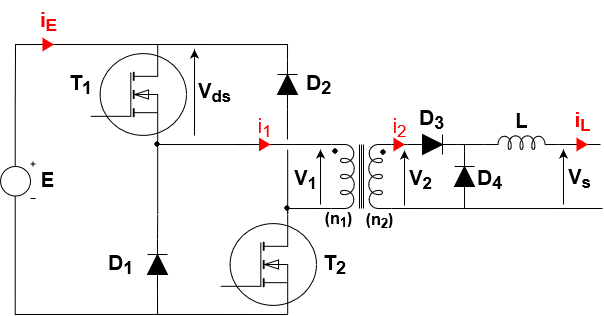
\includegraphics[width=0.85\linewidth]{TD_Forward_Asymetrique/fig/Forward_Asymetrique.png}
\end{figure}

\ifthenelse{\equal{\Langue}{FR}}{
Tous les semi-conducteurs sont supposés parfaits. Les deux bobinages du transformateur sont réalisés sur le même noyau ferromagnétique sans fuites: toutes les spires ``enlacent''  donc le même flux élémentaire $\varphi$, la réluctance de ce circuit magnétique étant notée $R$. La bobine d'inductance $L$ en sortie est indépendante de ce transformateur. Toutes les résistances sont négligées.

La commande des transistors est identique, réalisée à la période $T$, avec un rapport cyclique noté $\alpha$: ils sont donc conducteurs sur l'intervalle $[0,\ \alpha.T]$, bloqués sur l'intervalle $[\alpha.T,\ T]$.

La tension de sortie $V_s$ est supposée constante dans toute l'étude et le dispositif sera maintenu en démagnétisation totale à chaque cycle de fonctionnement. On ne s'intéresse qu'au régime de conduction continue dans l'inductance de sortie $L$, son courant ne s'annulant donc jamais: $i_L > 0$.
}{
All semiconductors are assumed to be perfect. The two windings of the transformer are made on the same ferromagnetic core without leakage: all the turns therefore ``enclose'' the same elementary flux $\varphi$, the reluctance of this magnetic circuit being denoted $R$. The output inductor $L$ is independent of this transformer. All resistances are neglected.

The control of the transistors is identical, carried out at the period $T$, with a duty cycle denoted $\alpha$: they are therefore conducting on the interval $[0,\ \alpha.T]$, blocked on the interval $[\alpha.T,\ T]$.

The output voltage $V_s$ is assumed to be constant throughout the study and the device will be maintained in total demagnetization at each operating cycle. We are only interested in the continuous conduction mode in the output inductor $L$, so its current never goes to zero: $i_L > 0$.

}
\begin{enumerate}
\ifthenelse{\equal{\Langue}{FR}}{
\item \textbf{Fonctionnement général de l'alimentation}
}{
\item \textbf{General operation of the power supply}
}

\ifthenelse{\equal{\Langue}{FR}}{
Dans cette partie, nous allons étudier le fonctionnement de l'alimentation. On supposera qu'elle fonctionne en \textbf{démagnétisation totale}, c'est à dire qu'à la fin d'une période, le flux magnétique dans le transformateur est nul. On tracera au fur et à mesure les courbes temporelles de $\varphi$ (flux magnétique dans le transformateur), $v_1$, $v_2$, $v_{DS}$ (tension drain-source du transistor $T_1$), $v_L$, $i_1$, $i_2$, $i_L$, et $i_E$.
}{
In this part, we will study the operation of the power supply. We will assume that it operates in \textbf{total demagnetization}, meaning that at the end of a period, the magnetic flux in the transformer is zero. We will plot the time curves of $\varphi$ (magnetic flux in the transformer), $v_1$, $v_2$, $v_{DS}$ (drain-source voltage of transistor $T_1$), $v_L$, $i_1$, $i_2$, $i_L$, and $i_E$.
}

\begin{enumerate}
\ifthenelse{\equal{\Langue}{FR}}{
\item Compte tenu des sens des enroulements représentés sur le schéma et des sens de mesure des différents courants et tensions:
}{
\item Considering the directions of the windings shown in the diagram and the directions of measurement of the different currents and voltages:
}
\begin{enumerate}
\ifthenelse{\equal{\Langue}{FR}}{
\item Donner l'expression des tensions $v_1$ et $v_2$ en fonction du flux $\varphi$
}{
\item Give the expression of the voltages $v_1$ and $v_2$ as a function of the flux $\varphi$
}

\ifthenelse{\equal{\SuCorr}{CO}}{
$v_1 = + n_1 \dfrac{d\varphi}{dt}$ \ hspace{1cm} $v_2 = + n_2 \dfrac{d\varphi}{dt}$
}

\ifthenelse{\equal{\Langue}{FR}}{
\item Exprimer la relation d'Hopkinson liant les courants $i_1$ et $i_2$ à ce même flux $\varphi$ au moyen des nombres de spires et de la réluctance $R$.
}{
\item Express the Hopkinson's law relating the currents $i_1$ and $i_2$ to the same flux $\varphi$ using the number of turns and the reluctance $R$.
}

\ifthenelse{\equal{\SuCorr}{CO}}{
$n_1 i_1 - n_2 i_2 = R . \varphi$
}

\end{enumerate}

\ifthenelse{\equal{\Langue}{FR}}{
\item On se place sur l'intervalle $[0,\ \alpha T]$: on suppose que le flux initial à t = 0 est nul (démagnétisation totale)
}{
\item We consider the interval $[0,\ \alpha T]$: we assume that the initial flux at $t = 0$ is zero (total demagnetization)
}
\begin{enumerate}
\ifthenelse{\equal{\Langue}{FR}}{
\item Déterminer la tension $v_1$ appliquée au bobinage primaire
}{
\item Determine the voltage $v_1$ applied to the primary winding
}

\ifthenelse{\equal{\SuCorr}{CO}}{
$0 < t < \alpha T$:

\begin{minipage}{0.45\linewidth}
\centering
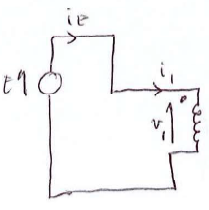
\includegraphics[width=\linewidth]{TD_Forward_Asymetrique/fig/0aT_schema_input.png}
\end{minipage}
\begin{minipage}{0.45\linewidth}
\centering
\ifthenelse{\equal{\Langue}{FR}}{$T_1$ et $T_2$ sont ``fermés''}{$T_1$ and $T_2$ are ``closed''}: 

$v_1 = E$
\end{minipage}

}

\ifthenelse{\equal{\Langue}{FR}}{
\item En déduire la tensions $v_2$ ainsi que l'état des diodes $D3$ et $D4$
}{
\item Deduce the voltage $v_2$ as well as the state of diodes $D3$ and $D4$
}

\ifthenelse{\equal{\SuCorr}{CO}}{
\begin{figure}[ht]
\centering
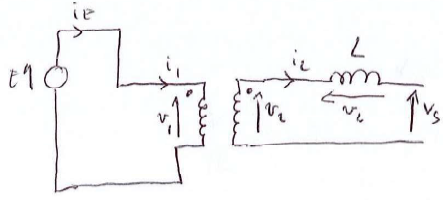
\includegraphics[width=0.75\linewidth]{TD_Forward_Asymetrique/fig/0aT_schema.png}
\end{figure}

$v_2 = \dfrac{n_2}{n_1} E > 0$ $\Rightarrow$ \ifthenelse{\equal{\Langue}{FR}}{$D3$ est passante et $D4$ est bloquée}{$D3$ is forward and $D4$ is reverse}
}

\ifthenelse{\equal{\Langue}{FR}}{
\item Donner l'expression de la tension $v_L$ aux bornes de l'inductance de sortie en fonction des nombres de spires, de $E$ et $V_S$
}{
\item Give the expression of the voltage $v_L$ across the output inductance in terms of the number of turns, $E$, and $V_S$
}

\ifthenelse{\equal{\SuCorr}{CO}}{
$v_L = v_2 - V_S = \dfrac{n_2}{n_1} E - V_S$
}

\ifthenelse{\equal{\Langue}{FR}}{
\item Exprimer l'évolution du flux $\varphi (t)$ sur cet intervalle de temps
}{
\item Express the evolution of the flux $\varphi (t)$ during this time interval
}

\ifthenelse{\equal{\SuCorr}{CO}}{
$v_1 = E = n_1 \dfrac{d\varphi}{dt} \Rightarrow \varphi (t) = \dfrac{E}{n_1} t + cste$

\ifthenelse{\equal{\Langue}{FR}}{A}{At} $t = 0$, $\varphi (0) = 0 \Rightarrow cste = 0$

$\varphi (t) = \dfrac{E}{n_1} t$
}


\ifthenelse{\equal{\Langue}{FR}}{
\item Exprimer le courant $i_2$ en fonction de $i_L$
}{
\item Express the current $i_2$ in terms of $i_L$
}

\ifthenelse{\equal{\SuCorr}{CO}}{
$i_2 = i_L$
}

\ifthenelse{\equal{\Langue}{FR}}{
\item A partir de la relation d'Hopkinson et des résultats précédents, déterminer l'expression du courant primaire $i_1$ en fonction de $i_L$ et du flux $\varphi$ au moyen des nombres de spires et de la réluctance $R$
}{
\item Using the Hopkinson's law and the previous results, determine the expression of the primary current $i_1$ in terms of $i_L$ and the flux $\varphi$ using the number of turns and the reluctance $R$
}

\ifthenelse{\equal{\SuCorr}{CO}}{
$n_1 i_1 - n_2 i_2 = R . \varphi \Rightarrow i_1 = \dfrac{n_2}{n_1} i_L + \dfrac{R}{n_1} \varphi$
}

\ifthenelse{\equal{\Langue}{FR}}{
\item A l'instant $\alpha T$, fin de ce premier intervalle de temps, on suppose que le flux est devenu égal à $\varphi_0$. En déduire l'expression de cette valeur de $\varphi_0$ en fonction de $E$, $n_1$ et $\alpha T$
}{
\item At the instant $\alpha T$, the end of this first time interval, we assume that the flux has become equal to $\varphi_0$. Deduce the expression of this value of $\varphi_0$ in terms of $E$, $n_1$, and $\alpha T$
}

\ifthenelse{\equal{\SuCorr}{CO}}{
$\varphi_0 = \varphi(\alpha T) = \dfrac{E}{n_1} \alpha T$
}

\end{enumerate}

\ifthenelse{\equal{\Langue}{FR}}{
\item On se place sur l'intervalle $[\alpha T,\ T]$: tous les transistors sont bloqués. 
}{
\item We consider the interval $[\alpha T,\ T]$: all transistors are blocked.
}
\begin{enumerate}
\ifthenelse{\equal{\Langue}{FR}}{
\item A $t=\alpha T$, déterminer l'état des diodes $D1$ et $D2$. Quelle sont les valeurs des tensions $v_1$ et $v_2$? En déduire l'état des diodes $D3$ et $D4$
}{
\item At $t=\alpha T$, determine the state of diodes $D1$ and $D2$. What are the values of voltages $v_1$ and $v_2$? Deduce the state of diodes $D3$ and $D4$
}

\ifthenelse{\equal{\SuCorr}{CO}}{
$\alpha T < t < T$: \ifthenelse{\equal{\Langue}{FR}}{$T_1$ et $T_2$ sont ``ouverts''}{$T_1$ and $T_2$ are ``opened''}
\ifthenelse{\equal{\Langue}{FR}}{A}{At} $t = \alpha T^+$, $\varphi(\alpha T^+) = \varphi_0$ (\ifthenelse{\equal{\Langue}{FR}}{Continuité du flux}{Flux continuity})

\ifthenelse{\equal{\Langue}{FR}}{De plus}{Furthermore}, $i_2>=0$ (\ifthenelse{\equal{\Langue}{FR}}{Courant dans la diode $D3$}{Current in diode $D3$}) 

$n_1 i_1 - n_2 i_2 = R . \varphi \Rightarrow i_1 = \dfrac{n_2}{n_1} i_2 + \dfrac{R}{n_1} \varphi >0$ 

$\Rightarrow$ \ifthenelse{\equal{\Langue}{FR}}{$D1$ et $D2$ sont passantes}{$D1$ and $D2$ are forward}

\begin{minipage}{0.45\linewidth}
\centering
\includegraphics[width=\linewidth]{TD_Forward_Asymetrique/fig/aTT_schema_input.png}
\end{minipage}
\begin{minipage}{0.45\linewidth}
\centering
$v_1 = -E$

$v_2 = -\dfrac{n_2}{n_1} E < 0$

$\Rightarrow$ \ifthenelse{\equal{\Langue}{FR}}{$D3$ est bloquée et $D4$ est passante}{$D3$ is reverse and $D4$ is forward}
\end{minipage}

}

\ifthenelse{\equal{\Langue}{FR}}{
\item En déduire l'expression de $v_L$ en fonction de $V_S$
}{
\item Deduce the expression of $v_L$ in terms of $V_S$
}

\ifthenelse{\equal{\SuCorr}{CO}}{
\begin{figure}[ht]
\centering
\includegraphics[width=0.75\linewidth]{TD_Forward_Asymetrique/fig/aTT_schema.png}
\end{figure}

$v_L = v_2 - V_S = - V_S$
}

\ifthenelse{\equal{\Langue}{FR}}{
\item Exprimer l'évolution du flux $\varphi(t)$ sur cet intervalle de temps
}{
\item Express the evolution of the flux $\varphi(t)$ during this time interval
}

\ifthenelse{\equal{\SuCorr}{CO}}{
$\varphi(\alpha T) = \varphi_0$

$v_1 = -E = n_1 \dfrac{d\varphi}{dt} \Rightarrow \varphi (t) = -\dfrac{E}{n_1} (t - \alpha T) + \varphi_0$
}

\ifthenelse{\equal{\Langue}{FR}}{
\item A quel instant $t_0$ le flux s'annule? Donner une condition sur $\alpha$ pour que le système fonctionne en démagnétisation totale
}{
\item At what instant $t_0$ does the flux become zero? Give a condition on $\alpha$ for the system to operate in total demagnetization
}

\ifthenelse{\equal{\SuCorr}{CO}}{
$\varphi(t_0) = 0 \Rightarrow t_0 = \alpha T + \dfrac{n_1}{E} \varphi_0 = 2 \alpha T$
}

\ifthenelse{\equal{\Langue}{FR}}{
\item Que se passe-t-il ensuite jusqu'à la fin de la période T\@?
}{
\item What happens next until the end of the period T\@?
}

\ifthenelse{\equal{\SuCorr}{CO}}{
\begin{itemize}
\item \ifthenelse{\equal{\Langue}{FR}}{Si $D_1$ et $D_2$ sont passantes}{If $D_1$ and $D_2$ are forward}:

$v_1 = -E \Rightarrow \varphi \searrow \Rightarrow \varphi <0$

$n_2 i_2 = n_1 i_1 - R \varphi > 0 \rightarrow D_3$ \ifthenelse{\equal{\Langue}{FR}}{passante}{forward}

\ifthenelse{\equal{\Langue}{FR}}{Or}{But} $v_2 = -\dfrac{n_2}{n_1} E < 0 \Rightarrow D_4$ \ifthenelse{\equal{\Langue}{FR}}{passante}{forward} $\Rightarrow v_2=0$ Contradiction

\end{itemize}

$\Rightarrow D_1$ \ifthenelse{\equal{\Langue}{FR}}{et}{and} $D_2$ \ifthenelse{\equal{\Langue}{FR}}{bloquées}{reverse} 

$\varphi$ constant

$i_1 = i_2 = 0$

$v_1 = v_2 = 0$
}

\end{enumerate}

\ifthenelse{\equal{\Langue}{FR}}{
\item L'alimentation est destinée à fabriquer une tension constante de valeur 24 V à partir du réseau monophasé redressé parfaitement filtré, $E = 300 V$. La puissance transmise est $P_n = 600 W$, la fréquence de découpage est $f = 50 kHz$. On choisit de faire fonctionner l'alimentation autour du rapport cyclique nominal $\alpha = 0.4$.
}{
\item The power supply is intended to produce a constant voltage of 24 V from the perfectly filtered single-phase rectified network, $E = 300 V$. The transmitted power is $P_n = 600 W$, and the switching frequency is $f = 50 kHz$. We choose to operate the power supply around the nominal duty cycle $\alpha = 0.4$.
}
\begin{enumerate}
\ifthenelse{\equal{\Langue}{FR}}{
\item Calculer le rapport de transformation $n_2/n_1$
}{
\item Calculate the turns ratio $n_2/n_1$
}

\ifthenelse{\equal{\SuCorr}{CO}}{
$<v_L> = 0 \Rightarrow (\dfrac{n_2}{n_1} E - V_S)\alpha -V_S(1-\alpha) = 0$

$\Rightarrow \dfrac{n_2}{n_1} = \dfrac{V_S}{\alpha E} = 0.2$
}

\ifthenelse{\equal{\Langue}{FR}}{
\item Calculer la valeur moyenne $I_s$ du courant $i_L$
}{
\item Calculate the average value $I_s$ of the current $i_L$
}

\ifthenelse{\equal{\SuCorr}{CO}}{
$P_S = V_S I_s \Rightarrow I_s = \dfrac{P_S}{V_S} = 25\ A$
}

\ifthenelse{\equal{\Langue}{FR}}{
\item Calculer la valeur minimale à donner à l'inductance $L$ pour limiter l'ondulation crête à crête du courant $i_L$ à 5\% de sa valeur moyenne $I_s$.\ \underline{On gardera cette} \underline{valeur de $L$ par la suite}
}{
\item Calculate the minimum value to be given to the inductance $L$ to limit the peak-to-peak ripple of the current $i_L$ to 5\% of its average value $I_s$.\ \underline{Keep this} \underline{value of $L$ for the following calculations}
}

\ifthenelse{\equal{\SuCorr}{CO}}{
$\alpha T < t < T$: $v_L = -V_S = L \dfrac{di_L}{dt} \Rightarrow \dfrac{di_L}{dt} = -\dfrac{V_S}{L}$
\
$\Delta i_L = \dfrac{V_S(1-\alpha)T}{L \Delta i_L} \Rightarrow L = \dfrac{V_S(1-\alpha)}{f\Delta i_L} = 0.23 mH$ 
}

\ifthenelse{\equal{\Langue}{FR}}{
\item En déduire la valeur maximale $I_{1\ \max}$ du courant dans le transistor lorsque l'on néglige le courant magnétisant
}{
\item Deduce the maximum value $I_{1\ \max}$ of the current in the transistor when neglecting the magnetizing current
}

\ifthenelse{\equal{\SuCorr}{CO}}{
$I_{1\ \max} = i_1(\alpha T) = \dfrac{n_2}{n_1} i_L(\alpha T) + \dfrac{R}{n_1} \varphi(\alpha T) \approx \dfrac{n_2}{n_1} i_L(\alpha T)$

$I_{1\ \max} = \dfrac{n_2}{n_1} 1.025 I_s =5.1\ A$
}

\end{enumerate}

\end{enumerate}

\ifthenelse{\equal{\Langue}{FR}}{
\item \textbf{Dimensionnement du transformateur}
}{
\item \textbf{Transformer sizing}
}
\begin{enumerate}
\ifthenelse{\equal{\Langue}{FR}}{
\item Pour justifier l'hypothèse précédente, déterminer la valeur minimale de l'inductance magnétisante $L_1$ (vue du bobinage au primaire) rendant le courant à vide maximal inférieur à $I_{1\ \max} /20$
}{
\item To justify the previous assumption, determine the minimum value of the magnetizing inductance $L_1$ (seen from the primary winding) that makes the maximum no-load current less than $I_{1\ \max} /20$
}

\ifthenelse{\equal{\SuCorr}{CO}}{
$0 < t < \alpha T$: $v_1 = E = L_1 \dfrac{di_m}{dt}$

$I_{m\ \max} = i_m(\alpha T) = \dfrac{E}{L_1} \alpha T < \dfrac{I_{1\ \max}}{20}$

$\Rightarrow L_1 > \dfrac{20 E \alpha T}{I_{1\ \max}} = 9.4\ mH$
}

\ifthenelse{\equal{\Langue}{FR}}{
\item \underline{En négligeant l'ondulation du courant $i_L$ et le courant magnétisant}, déterminer les valeurs efficaces $I_{1\ eff}$ et
$I_{2\ eff}$ des courants $i_1$ et $i_2$ en fonction de $I_s$, $n_1$, $n_2$ et $\alpha$
}{
\item \underline{Neglecting the ripple of the current $i_L$ and the magnetizing current}, determine the rms values $I_{1\ eff}$ and
$I_{2\ eff}$ of the currents $i_1$ and $i_2$ in terms of $I_s$, $n_1$, $n_2$, and $\alpha$
}

\ifthenelse{\equal{\SuCorr}{CO}}{
\begin{itemize}
\item $0 < t < \alpha T$: 

$i_1 = \dfrac{n_2}{n_1} i_S$

$i_2=I_S$
\item $\alpha T < t < T$:

$i_1 = 0$

$i_2=0$
\end{itemize}
$\Rightarrow I_{1\ eff} = \dfrac{n_2}{n_1} I_S \sqrt{\alpha}$

$I_{2\ eff} = I_S \sqrt{\alpha}$
}

\ifthenelse{\equal{\Langue}{FR}}{
\item Déterminer, avec ces mêmes hypothèses, la surface de bobinage minimale nécessaire $S_B$ en fonction de $\delta$ (densité de courant), $k_B$ (coefficient de bobinage), $I_s$, $n_2$ et $\alpha$
}{
\item Determine, with these same assumptions, the minimum winding area $S_B$ required in terms of current density $\delta$, winding coefficient $k_B$, $I_s$, $n_2$, and $\alpha$
}

\ifthenelse{\equal{\SuCorr}{CO}}{
$S_B = \dfrac{S_{TCu}}{\delta k_B} = \dfrac{1}{\delta k_B} (n_1 I_{1\ eff} + n_2 I_{2\ eff})$

$S_B = \dfrac{1}{\delta k_B} \left(n_2 I_S \sqrt{\alpha} + n_2 I_S \sqrt{\alpha}\right) = \dfrac{2 n_2 I_S \sqrt{\alpha}}{\delta k_B}$
}

\ifthenelse{\equal{\Langue}{FR}}{
\item Donner également l'expression de la section minimale $A_e$ du noyau permettant d'éviter la saturation du noyau en maintenant une induction maximale inférieure à $B_{\max}$
}{
\item Also give the expression of the minimum cross-sectional area $A_e$ of the core that avoids core saturation by maintaining a maximum induction below $B_{\max}$
}

\ifthenelse{\equal{\SuCorr}{CO}}{
$\varphi_{\max} = B_{\max} A_e = \dfrac{E}{n_1} \alpha T$

$\Rightarrow A_{e \min} = \dfrac{E \alpha}{n_1 f B_{\max}}$
}

\ifthenelse{\equal{\Langue}{FR}}{
\item En déduire le produit de dimensionnement $A_e.S_B$ minimal de ce transformateur en fonction du rapport cyclique, des différents paramètres caractéristiques de cette alimentation, notamment sa puissance de sortie $P_S$ et sa fréquence de découpage $f$
}{
\item Deduce the minimal sizing product $A_e.S_B$ of this transformer in terms of the duty cycle, the different characteristic parameters of this power supply, including its output power $P_S$, and its switching frequency $f$
}

\ifthenelse{\equal{\SuCorr}{CO}}{
$A_e.S_B > \dfrac{2 n_2 E \alpha I_S \sqrt{\alpha}}{n_1 f B_{\max} \delta k_B} = \dfrac{2 V_S I_S \sqrt{\alpha}}{f B_{\max} \delta k_B} = \dfrac{2 P_S \sqrt{\alpha}}{f B_{\max} \delta k_B}$
}

\end{enumerate}

\end{enumerate}

\begin{figure}[ht]
\centering
\ifthenelse{\equal{\SuCorr}{CO}}{
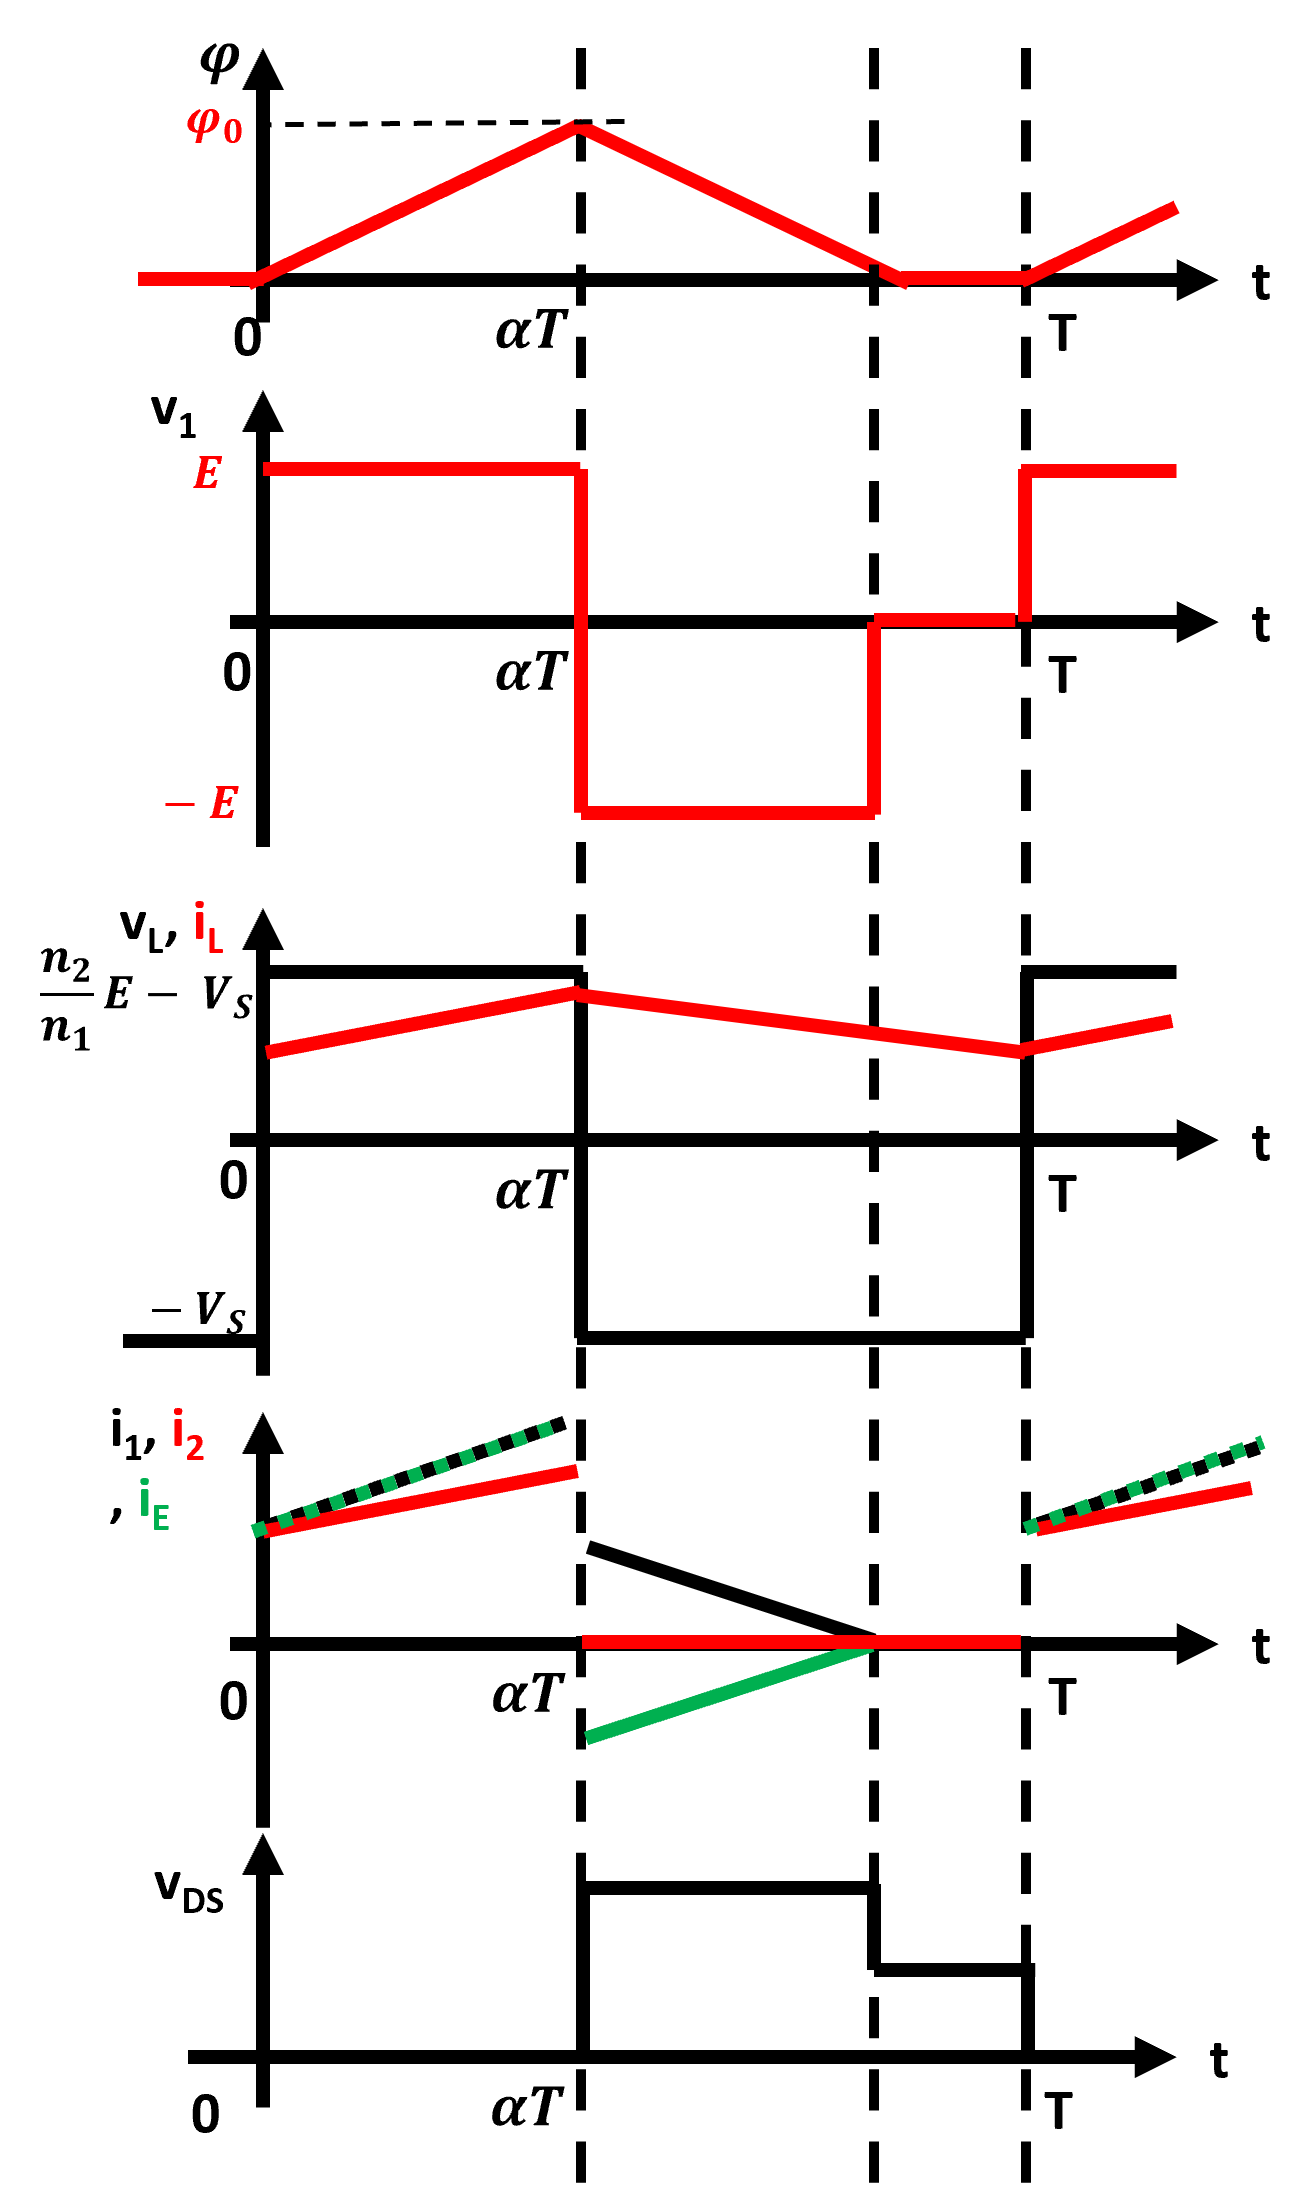
\includegraphics[width=0.84\linewidth]{TD_Forward_Asymetrique/fig/doc_reponse_corrige.png}
}{
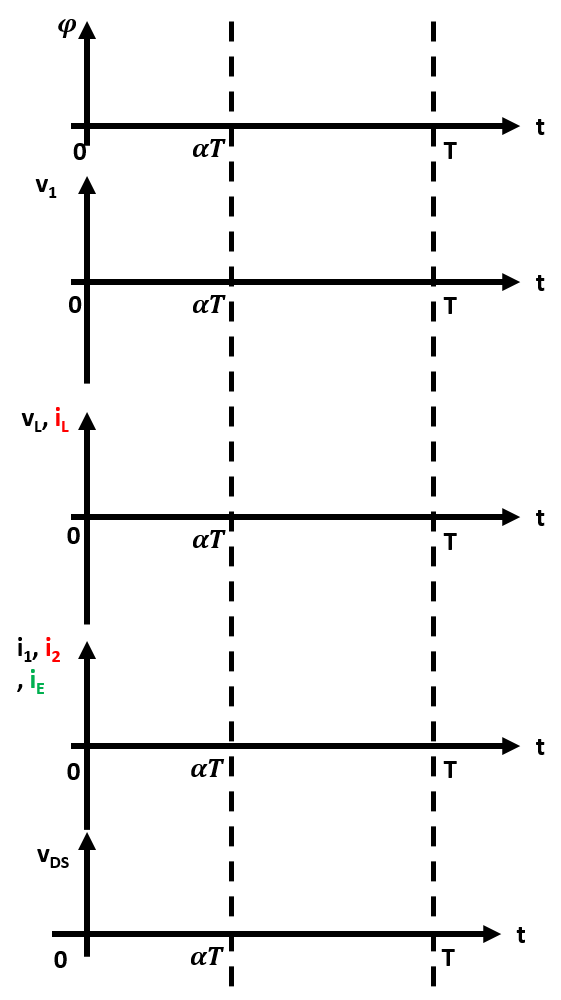
\includegraphics[width=0.84\linewidth]{TD_Forward_Asymetrique/fig/doc_reponse.png}
}
\end{figure}
